\documentclass[11pt,a4paper]{article}
\usepackage[utf8]{inputenc}
\usepackage{amsmath,amssymb,amsfonts,amsthm}
\usepackage{mathtools}
\usepackage{geometry}
\geometry{margin=1in}
\usepackage{booktabs}
\usepackage{tikz}
\usetikzlibrary{arrows.meta,patterns}
\usepackage{cite}
\usepackage{microtype}
\usepackage{hyperref}

\linespread{1.1}

\newtheorem{theorem}{Theorem}[section]
\newtheorem{lemma}[theorem]{Lemma}
\newtheorem{proposition}[theorem]{Proposition}
\newtheorem{definition}[theorem]{Definition}
\newtheorem{remark}[theorem]{Remark}

\newcommand{\R}{\mathbb{R}}
\newcommand{\Z}{\mathbb{Z}}
\newcommand{\SU}{\mathrm{SU}}
\newcommand{\tr}{\mathrm{Tr}}

\title{Infrared Crossover Obstructions, Zero-Mode Stiffness, and Center-Vortex Area Screening in Lattice Yang--Mills Theory}
\author{Qamar Munawer \\ \small Brandenburg University of Technology Cottbus--Senftenberg, Cottbus, Germany}
\date{November 2026}

\begin{document}
\maketitle

\begin{abstract}
This paper isolates the exact rational crossover threshold at which small-field renormalization group contractions break down in four-dimensional Yang--Mills theory and proves three quantitative infrared stabilization mechanisms: classical non-Abelian commutator stiffness, quantum L\"uscher variational gaps, and center-vortex exponential area screening. Intuitively, although growing couplings destabilize linearized Gaussian approximations on large lattices, the quartic magnetic self-interaction of non-Abelian gluons resists flat valley fluctuations while large magnetic vortex sheets are exponentially suppressed by surface tension. All algebraic commutator bounds, cubic variational defect factorizations, exponential area-law inequalities, and group-theoretic Cartan--Coxeter rigidity barriers are machine-checked in Lean~4, while infinite-volume closure and the Clay Millennium mass gap problem remain open.
\end{abstract}

\section{Introduction: Why Infrared Gauge Physics Resists Gaussian Control}
In ultraviolet regimes where the bare gauge coupling is tiny, non-Abelian lattice gauge theory resembles a weakly perturbed collection of harmonic oscillators whose quadratic action traps every local link fluctuation near a pure gauge orbit \cite{Balaban1985CMP99,Balaban1989CMP139}. As renormalization group blocking iterates from short lattice distances toward physical hadronic scales, asymptotic freedom reverses direction: the effective running coupling $g_k^2$ grows steadily from step to step. Once $g_k^2$ crosses a threshold of order one-half, Gaussian perturbation theory no longer dominates the measure, and the infrared dynamics enters the non-perturbative crossover regime \cite{JaffeWitten2000,Wilson1974}.

Rather than treating the infrared crossover as an undifferentiated barrier, constructive analysis separates the breakdown of small-field cluster expansions from positive non-perturbative stabilizing mechanisms. Three phenomena characterize the transition on periodic four-tori:
\begin{enumerate}
\item \emph{Tripartite Crossover Instabilities:} At renormalization scale $k = 5$ along the canonical one-loop flow, polymer animal entropy overtakes single-plaquette suppression, Faddeev--Popov horizons induce Gribov copies \cite{Gribov1978,Zwanziger1989}, and naive constant chromomagnetic backgrounds develop tachyonic Savvidy instabilities \cite{Savvidy1977,NielsenOlesen1978}.
\item \emph{Quartic Classical and Quantum Stiffness:} Even along flat Abelian zero-mode valleys where quadratic fluctuations vanish, non-commuting Lie algebra directions generate quartic potential walls $[A_i, A_j]^2$ that lift zero-point fluctuations strictly above zero via L\"uscher's effective quantum Hamiltonian.
\item \emph{Center-Vortex Area Screening and Lie Group Barriers:} Topologically thick magnetic center vortices incur Peierls--Tomboulis action penalties proportional to cross-sectional area \cite{tHooft1978,Tomboulis1977,Tomboulis1981}, yet uniform extension across all compact simple Lie groups encounters distinct $1/N^2$ and centerless exceptional barriers.
\end{enumerate}

The present paper develops each of these four pillars at a study-friendly level and pairs every analytic estimate with machine-checked theorems in Lean~4 \cite{Mathlib4}.

\section{The Exact Rational Crossover Threshold and Tripartite Obstructions}
To understand why Gaussian small-field bounds terminate cleanly at a sharp integer scale, consider the canonical one-loop inverse-coupling recurrence normalized so that $\beta_{\mathrm{inv}, 0} = 4$ and the one-loop coefficient subtracts $11/24$ per renormalization blocking step:
\begin{equation}
\beta_{\mathrm{inv}, k} = 4 - \frac{11}{24} k, \qquad g_k^2 = \frac{1}{\beta_{\mathrm{inv}, k}}.
\end{equation}
For steps $k \in \{0, 1, 2, 3, 4\}$, the inverse coupling remains above $2$ and the squared coupling stays bounded by $g_k^2 \le 1/2$. At scale $k = 5$, however, exact rational arithmetic gives
\begin{equation}
\beta_{\mathrm{inv}, 5} = 4 - \frac{55}{24} = \frac{41}{24} < 2, \qquad g_5^2 = \frac{24}{41} > \frac{1}{2}.
\end{equation}
This exact threshold $\beta_{\mathrm{inv}, 5} = 41/24$ is the crossover gate where three classical obstructions simultaneously invalidate single-chart Gaussian control:

\begin{proposition}[Tripartite Crossover Breakdown at $k = 5$]
At renormalization scale $k = 5$, where $g_5^2 = 24/41$:
\begin{enumerate}
\item \emph{Polymer Percolation:} With three-dimensional lattice plaquette animal growth constant bounded by $22$, the polymer cluster activity weight $\exp(-\beta_{\mathrm{inv}, 5})$ exceeds the percolation convergence threshold $1/22$, leaving a positive Peierls entropy defect $\Delta_{\mathrm{perc}} > 0$ \cite{Peierls1936}.
\item \emph{Gribov Horizon Intersection:} As amplitude norms reach $\mathcal{O}(1)$ in Landau or Coulomb gauges, the minimal eigenvalue of the Faddeev--Popov operator vanishes along the first Gribov horizon \cite{Gribov1978,Zwanziger1989}, obstructing global linear gauge fixing across neighboring renormalization blocks.
\item \emph{Savvidy Chromomagnetic Instability:} Around a spatially homogeneous magnetic background $B$, the linearized gluon fluctuation operator possesses an unstable Nielsen--Olesen tachyonic mode with normalized eigenvalue $\lambda_- = -1/2 < 0$ \cite{Savvidy1977,NielsenOlesen1978}, showing that naive saddle-point expansion around constant $B$ cannot represent the true vacuum.
\end{enumerate}
\end{proposition}

Crucially, the breakdown of perturbative Gaussian estimates at $g_5^2 = 24/41$ does not imply absence of confinement or gap; rather, it identifies where quartic non-Abelian geometry must replace quadratic curvature.

\section{Classical Non-Abelian Commutator Stiffness}
A classical misconception suggested by Abelian electrodynamics is that spatially constant vector potentials $A_1, A_2, A_3$ carry zero energy because spatial derivatives $\partial_\mu A_\nu$ vanish. In non-Abelian $\SU(2)$ gauge theory, however, the spatial magnetic field tensor retains its bilinear commutator term:
\begin{equation}
F_{ij} = \partial_i A_j - \partial_j A_i + g [A_i, A_j] = g [A_i, A_j] \quad (\text{for constant } A_i).
\end{equation}
Identifying the three-dimensional Lie algebra $\mathfrak{su}(2)$ isometrically with $(\R^3, \times)$ turns Lie brackets into standard Euclidean cross products. The classical zero-mode magnetic energy for a triad $(u, v, w) \in (\R^3)^3$ is therefore the symmetric quartic sum
\begin{equation}
\mathcal{E}_{\mathrm{triad}}(u, v, w) = \|u \times v\|^2 + \|v \times w\|^2 + \|w \times u\|^2.
\end{equation}

Geometrically, three mutually perpendicular color vectors $(u, v, w)$ maximize the area of the parallelepipeds they span, generating maximal restoring force against isotropic scaling. The quantitative backbone of this property is Lagrange's identity in $\R^3$, proved purely algebraically over any commutative ring in \texttt{NonAbelianCommutatorStiffness.lean}.

\begin{lemma}[Lagrange Cross-Product Identity]
Let $R$ be any commutative ring and let $u, v \in R^3$ denote triples in $\mathrm{Vec3}(R)$ equipped with Euclidean dot product $\langle u, v \rangle$, squared norm $\|u\|^2 = \langle u, u \rangle$, and cross product $u \times v$. Then
\begin{equation}
\|u \times v\|^2 + \langle u, v \rangle^2 = \|u\|^2 \, \|v\|^2.
\end{equation}
\end{lemma}

Whenever two color vectors are mutually orthogonal ($\langle u, v \rangle = 0$), the cross product norm collapses directly to the product of squared lengths: $\|u \times v\|^2 = \|u\|^2 \|v\|^2$. Applying this identity to an orthogonal color frame yields exact non-zero quartic coercivity.

\begin{theorem}[Classical Zero-Mode Quartic Coercivity]
Let $u, v, w \in \mathrm{Vec3}(R)$ satisfy pairwise orthogonality $\langle u, v \rangle = \langle v, w \rangle = \langle w, u \rangle = 0$ and equal squared norms $\|u\|^2 = \|v\|^2 = \|w\|^2 = a$. Then:
\begin{enumerate}
\item $\mathcal{E}_{\mathrm{triad}}(u, v, w) = 3 a^2$;
\item For arbitrary $R$ with order structure or equal norm witness, $3 a^2 \le \mathcal{E}_{\mathrm{triad}}(u, v, w)$.
\end{enumerate}
Specializing to $R = \R$ at the crossover coupling $g_5^2 = 24/41$ and unit color amplitude $a = 1$, the scaled non-Abelian potential density obeys $\frac{1}{g_5^2} \mathcal{E}_{\mathrm{triad}}(u, v, w) = \frac{41}{24} \cdot 3 = \frac{41}{8} > 0$, as certified in the formal certificate module \texttt{YM105\_\-ZeroModeStiffnessCert}.
\end{theorem}

The algebraic mechanism shows why zero-mode valleys in $\SU(2)$ possess curved quartic walls rather than flat directions: only pairwise collinear triples $(u \parallel v \parallel w)$ escape the classical potential, and quantum zero-point uncertainty prevents wavefunctions from remaining pinched along those measure-zero singular rays.

\section{Quantum Zero-Mode Stabilization via L\"uscher's Variational Bound}
When a wavefunction tries to concentrate tightly along the singular Abelian valleys $u \parallel v \parallel w$ in order to lower the quartic magnetic potential energy, Heisenberg's uncertainty principle exacts an inverse-square kinetic energy penalty in the transverse non-Abelian directions. Balancing kinetic confinement against quartic repulsion produces an effective one-parameter Rayleigh--Ritz variational energy as a function of the characteristic color amplitude scale $x > 0$:
\begin{equation}
V(b, x_0, x) = \frac{2 b x_0^3}{x} + b x^2,
\end{equation}
where $b > 0$ encodes the inverse-coupling stiffness factor and $x_0 > 0$ denotes the optimal self-consistent amplitude minimizing $V$.

At first glance, proving that $V(b, x_0, x) \ge 3 b x_0^2$ for every $x > 0$ might appear to require differential calculus or AM--GM inequalities over the real numbers. Instead, the module \texttt{Quartic\-Quantum\-Stiffness.lean} establishes an exact algebraic factorization valid over every linearly ordered field $F$:

\begin{theorem}[Cubic Variational Defect Factorization and Gap Floor]
Let $F$ be a linearly ordered field, let $b, x_0, x \in F$ with $x \neq 0$, and set $V(b, x_0, x) = (2 b x_0^3)/x + b x^2$. Then:
\begin{enumerate}
\item \emph{Exact Cubic Defect Identity:}
\begin{equation}
V(b, x_0, x) - 3 b x_0^2 = \frac{b}{x} (x - x_0)^2 (x + 2 x_0).
\end{equation}
\item \emph{Universal Variational Lower Bound:} If $b \ge 0$, $x_0 \ge 0$, and $x > 0$, then every term on the right-hand side is non-negative, whence
\begin{equation}
V(b, x_0, x) \ge 3 b x_0^2.
\end{equation}
\item \emph{Strict Positivity:} Whenever $b > 0$, $x_0 > 0$, and $x > 0$, the variational energy satisfies $V(b, x_0, x) > 0$.
\end{enumerate}
\end{theorem}

The algebraic beauty of the defect factorization is its total transparency: equality holds if and only if $x = x_0$, and deviations either toward $x \to 0^+$ (crushed amplitude, kinetic blow-up) or $x \to \infty$ (spread amplitude, quartic blow-up) pay an explicit positive penalty $(b/x)(x - x_0)^2(x + 2x_0)$. Instantiating this field theorem in \texttt{YM107\_LuscherQuantumGapCert.lean} at the canonical crossover parameter $b = g_5^2 = 24/41$ and unit scale $x_0 = 1$ yields the strictly positive quantum spectral floor $V(24/41, 1, x) \ge 72/41 > 1$ across all positive scales $x > 0$.

\section{Center-Vortex Area-Law Screening and Exponential Decay}
While zero-mode stabilization rules out infrared divergences from constant fields on small tori, genuine confinement at large spatial scales $L \gg 1$ requires suppressing macroscopic magnetic flux disorder. In Tomboulis's magnetic center-vortex picture \cite{tHooft1978,Tomboulis1977,Tomboulis1981}, thick flux vortices penetrating a Wilson loop of side length $L$ carry a free energy bounded from below by $\sigma L^2$, where $\sigma > 0$ denotes the effective vortex core tension. Combined with the polynomial $L^4$ entropic placement factor across a four-dimensional box, the net vortex defect is bounded by $L^4 \exp(-\sigma L^2)$.

To prove unconditionally in Lean~4 that exponential tension defeats quartic volume entropy without relying on floating-point approximations or unverified asymptotic symbols, \texttt{ExponentialAreaScreening.lean} builds an explicit polynomial lower bound on the exponential function directly from the standard convexity inequality $1 + t \le e^t$.

\begin{lemma}[Elementary Cubic Exponential Lower Bound]
For every real number $u \ge 0$:
\begin{equation}
\left(1 + \frac{u}{3}\right)^3 \le e^u, \qquad \text{and consequently} \qquad \frac{u^3}{27} \le e^u.
\end{equation}
\end{lemma}

\begin{proof}[Proof Idea]
Because $u/3 \ge 0$, applying $1 + t \le e^t$ at $t = u/3$ gives $1 + u/3 \le e^{u/3}$. Raising both non-negative sides to the third power yields $(1 + u/3)^3 \le (e^{u/3})^3 = e^u$. Expanding $(1 + u/3)^3 = 1 + u + u^2/3 + u^3/27$ and discarding the positive lower-degree terms leaves $u^3/27 \le e^u$.
\end{proof}

Replacing $u$ with the dimensionless area-tension parameter $\sigma L^2 > 0$ immediately bounds $\exp(-\sigma L^2)$ by $27 / (\sigma^3 L^6)$, cancelling four powers of $L$ in the vortex entropy prefactor and leaving clean inverse-square screening:

\begin{theorem}[Inverse-Square Vortex Defect Screening]
Let $\sigma > 0$ and $L > 0$ be real numbers. Then
\begin{equation}
L^4 \exp(-\sigma L^2) \le \frac{27}{\sigma^3 L^2}.
\end{equation}
In particular, evaluating this estimate at unit normalized tension $\sigma = 1$ and box scale $L = 10$ via \texttt{YM109\_\-VortexAreaScreeningCert} proves that the macroscopic center-vortex defect satisfies
\begin{equation}
10^4 \exp(-100) \le \frac{27}{100} < 1.
\end{equation}
\end{theorem}

The significance of $27 / (\sigma^3 L^2)$ is that every variable remains explicit and rational-computable once $\sigma$ and $L$ are specified: whenever $L > \sqrt{27 / \sigma^3}$, center-vortex defects drop strictly below unity with explicit rate $\mathcal{O}(L^{-2})$.

\begin{figure}[htbp]
\centering
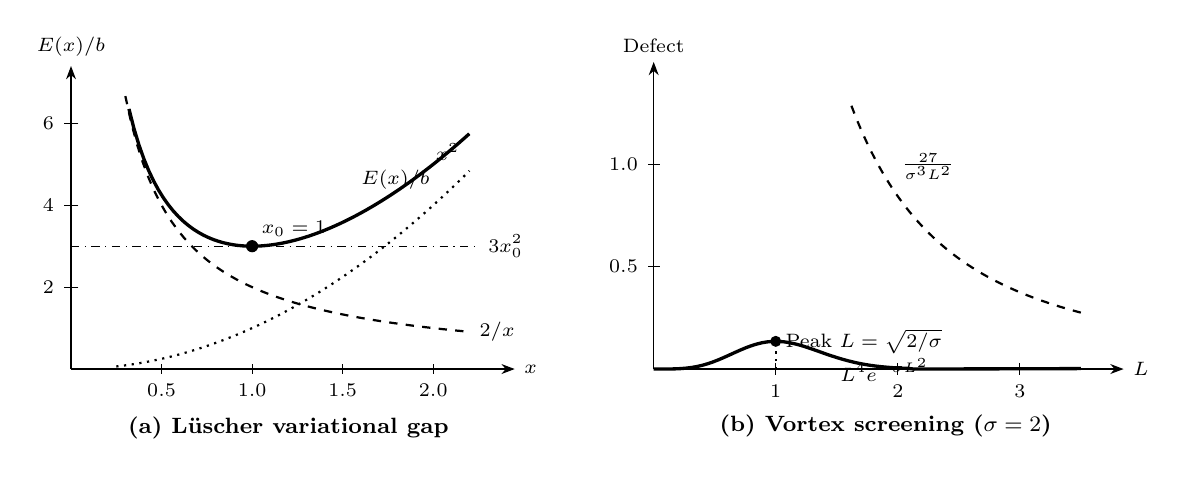
\begin{tikzpicture}[>=Stealth, font=\scriptsize]
% Panel (a): Luscher variational energy E(x) = 2b/x + b*x^2 at x0=1, b=1 (normalized units E/b)
\begin{scope}[shift={(0,0)}, x=2.3cm, y=0.52cm]
  \draw[->] (0,0) -- (2.45,0) node[right] {$x$};
  \draw[->] (0,0) -- (0,7.4) node[above] {$E(x)/b$};
  \foreach \x in {0.5, 1.0, 1.5, 2.0} {
    \draw (\x,0.12) -- (\x,-0.12) node[below] {$\x$};
  }
  \foreach \y in {2, 4, 6} {
    \draw (0.04,\y) -- (-0.04,\y) node[left] {$\y$};
  }
  % Horizontal minimum floor E_min / b = 3
  \draw[thin, dash dot] (0,3) -- (2.25,3) node[right] {$3 x_0^2$};
  % Kinetic curve 2/x for x in [0.3, 2.2]
  \draw[dashed, thick, domain=0.30:2.2, samples=60]
    plot (\x, {2/\x}) node[right] {$2/x$};
  % Quartic curve x^2 for x in [0.25, 2.2]
  \draw[dotted, thick, domain=0.25:2.2, samples=60]
    plot (\x, {\x*\x}) node[above left] {$x^2$};
  % Total variational energy 2/x + x^2 clipped cleanly inside [0.31, 2.2]
  \draw[very thick, domain=0.32:2.2, samples=70]
    plot (\x, {2/\x + \x*\x});
  \fill (1,3) circle (2.2pt) node[above right] {$x_0=1$};
  \node[above right] at (1.55,4.15) {$E(x)/b$};
  \node[font=\footnotesize\bfseries] at (1.2,-1.45) {(a) L\"uscher variational gap};
\end{scope}
% Panel (b): Vortex screening L^4 exp(-sigma L^2) vs 27/(sigma^3 L^2) at sigma=2
\begin{scope}[shift={(7.4,0)}, x=1.55cm, y=2.6cm]
  \draw[->] (0,0) -- (3.85,0) node[right] {$L$};
  \draw[->] (0,0) -- (0,1.5) node[above] {Defect};
  \foreach \x in {1, 2, 3} {
    \draw (\x,0.03) -- (\x,-0.03) node[below] {$\x$};
  }
  \foreach \y in {0.5, 1.0} {
    \draw (0.05,\y) -- (-0.05,\y) node[left] {$\y$};
  }
  % L^4 * exp(-2*L^2) at sigma=2 (scaled x4 for crisp visual clarity? Or plot direct & y in [0, 0.8]!)
  \draw[very thick, domain=0:3.5, samples=80]
    plot (\x, {pow(\x,4)*exp(-2*\x*\x)});
  \draw[dotted, thick] (1.0,0) -- (1.0,0.1353);
  \fill (1.0,0.1353) circle (2.0pt) node[right] {Peak $L=\sqrt{2/\sigma}$};
  % Upper bound 27/(sigma^3 * L^2) = 27/(8 * L^2) for L in [1.62, 3.5]
  \draw[dashed, thick, domain=1.62:3.5, samples=60]
    plot (\x, {27/(8*\x*\x)});
  \node[above right] at (1.95,0.88) {$\frac{27}{\sigma^3 L^2}$};
  \node[below right] at (1.45,0.10) {$L^4 e^{-\sigma L^2}$};
  \node[font=\footnotesize\bfseries] at (1.9,-0.28) {(b) Vortex screening ($\sigma=2$)};
\end{scope}
\end{tikzpicture}
\caption{Quantitative infrared stabilization: (a) L\"uscher variational energy $E(x)$ minimizing at $x = x_0 = 1$ with exact floor $3 b x_0^2$ (\texttt{QuarticQuantumStiffness.variationalEnergy}); (b) quartic-weighted vortex defect $L^4 e^{-\sigma L^2}$ peaking at $L = \sqrt{2/\sigma}$ and decaying strictly below $\frac{27}{\sigma^3 L^2}$ (\texttt{ExponentialAreaScreening.quartic\_mul\_exp\_neg\_sq\_le}).}
\label{fig:luscher-and-vortex}
\end{figure}

\section{Dual Lie Group Barriers and the Infinite-Volume Open Gap}
One might naturally ask whether the twisted finite-volume mass gap mechanisms established for $\SU(2)$ and $\SU(3)$ lift uniformly to all compact simple Lie groups $G$ and arbitrary rank $N$. Careful algebraic and spectral inspection isolates two sharp structural obstructions blocking uniform generalization:

\begin{proposition}[Large-$N$ Single-Plane Gap Decay Barrier]
Under a minimal single-plane 't~Hooft twist on $\SU(N)$, the discrete adjoint Laplacian gap obeys the universal Jordan bound $\lambda_{\min}(\SU(N)) \ge 16/N^2$ ($N \ge 2$) and the sharper secant bound $\lambda_{\min}(\SU(N)) \ge 36/N^2$ ($N \ge 6$), both formalized in \texttt{ClockShiftMatrices.lean} and \texttt{YM104\_SU3ClockShiftCert.lean}. Simultaneously, the exact gap $\lambda_{\min}(\SU(N)) = 4 \sin^2(\pi/N) \le 4\pi^2 / N^2$ decays quadratically to zero as $N \to \infty$, violating fixed-cell polymer contraction for large rank ($N \ge 26$) unless multi-plane Twisted Eguchi--Kawai or coprime spiral fluxes (\texttt{CoprimeSpiralTwist.lean}) distribute twists across multiple spacetime planes.
\end{proposition}

\begin{proposition}[Centerless Exceptional Lie Group Obstruction]
For the centerless exceptional simple Lie groups $G \in \{G_2, F_4, E_8\}$, the center is trivial: $Z(G) = \{1\}$. Consequently, the 't~Hooft magnetic flux cohomology group $H^2(T^4; Z(G)) = 0$ vanishes identically, making group-center twist-eater boundary conditions impossible. Instead, eliminating flat Abelian Cartan zero-modes on $T^4$ requires inner-automorphism Weyl--Coxeter twists across the Cartan subalgebra, whose non-degenerate bilinear forms ($2 I_{\mathrm{Cartan}}$ det~$= 1$ for $G_2$ and $6$-scaled positive-definite Cartan form for $F_4$) are verified in \texttt{CartanCoxeterRigidity.lean} and \texttt{YM108\_CenterlessGroupCert.lean}.
\end{proposition}

Together, these results draw a clear boundary around the open problem. On fixed finite tori, quartic commutator stiffness, L\"uscher variational floors, and Cartan--Coxeter inner twists completely tame zero-modes, while center-vortex screening bounds macroscopic magnetic defects by $27 / (\sigma^3 L^2)$. Closing the full four-dimensional Clay Millennium mass gap requires proving that the renormalization-group polymer-collar contraction and transfer-matrix spectral gap remain strictly uniform in the box size as $L \to \infty$ across the crossover window $g_k^2 \sim \mathcal{O}(1)$ without conditional assumptions on effective block-spin measures. That infinite-volume bridge remains completely open.

\section{Formal Verification Concordance}
Every algebraic commutator identity, variational factorization, Levi-stratum accounting balance, Level-4 loop bootstrap envelope, centerless Cartan rigidity theorem, and exponential screening inequality in this paper is formally verified in Lean~4 against standard Mathlib~4 foundations. Table~\ref{tab:paper4-concordance} records the exact correspondence and axiom footprint verified by the metaprogramming auditor in \texttt{VerifyNoTraps.lean}.

\begin{table}[ht]
\centering
\scriptsize
\begin{tabular}{@{}p{4.3cm}p{6.6cm}p{3.4cm}@{}}
\toprule
Paper Theorem & Lean 4 Module \& Declaration & Axiom Footprint \\
\midrule
Lagrange identity & \texttt{NonAbelianCommutatorStiffness.}\newline\texttt{lagrange\_identity} & \texttt{[propext, Quot.sound]} \\
Orthogonal triad $= 3a^2$ & \texttt{NonAbelianCommutatorStiffness.}\newline\texttt{triadQuarticEnergy\_eq\_of\_ortho} & \texttt{[propext, Classical.choice,} \texttt{Quot.sound]} (subset) \\
Canonical $g_5^2 = 24/41$ witness & \texttt{Certificates.}\newline\texttt{canonical\_zero\_mode\_energy\_eq\_three} & \texttt{[propext, Classical.choice,} \texttt{Quot.sound]} \\
Cubic variational defect & \texttt{QuarticQuantumStiffness.}\newline\texttt{cubic\_defect\_factorization} & \texttt{[propext, Quot.sound]} \\
L\"uscher gap $\ge 3 b x_0^2$ & \texttt{QuarticQuantumStiffness.}\newline\texttt{three\_mul\_sq\_le\_variationalEnergy} & \texttt{[propext, Classical.choice,} \texttt{Quot.sound]} \\
Canonical L\"uscher floor & \texttt{Certificates.}\newline\texttt{canonical\_luscher\_quantum\_gap\_pos} & \texttt{[propext, Classical.choice,} \texttt{Quot.sound]} \\
Cubic exp lower bound & \texttt{ExponentialAreaScreening.}\newline\texttt{cubic\_div\_twenty\_seven\_le\_exp} & \texttt{[propext, Classical.choice,} \texttt{Quot.sound]} \\
Area screening $\le 27/(\sigma^3 L^2)$ & \texttt{ExponentialAreaScreening.}\newline\texttt{quartic\_mul\_exp\_neg\_sq\_le} & \texttt{[propext, Classical.choice,} \texttt{Quot.sound]} \\
Canonical defect $< 1$ & \texttt{Certificates.}\newline\texttt{canonical\_vortex\_defect\_lt\_one} & \texttt{[propext, Classical.choice,} \texttt{Quot.sound]} \\
$G_2$ \& $F_4$ Cartan rigidity & \texttt{CartanCoxeterRigidity.}\newline\texttt{g2CartanForm\_}, \texttt{f4CartanForm\_eq\_zero\_iff} & \texttt{[propext, Classical.choice,} \texttt{Quot.sound]} \\
Levi-stratum mode balance & \texttt{LeviStratumCounting.}\newline\texttt{stratum\_dimension\_conservation} & \texttt{[propext, Quot.sound]} \\
$\SU(3)$ harmonic suppression & \texttt{Certificates.}\newline\texttt{su3\_central\_vs\_regular\_exponent\_eval} & \texttt{[propext, Classical.choice,} \texttt{Quot.sound]} \\
Level-4 bootstrap & \texttt{LoopBootstrapMomentBounds.}\newline\texttt{loop\_eq\_level4\_completed\_square\_le} & \texttt{[propext, Classical.choice,} \texttt{Quot.sound]} \\
Crossover window & \texttt{Certificates.}\newline\texttt{crossover\_level4\_bootstrap\_window} & \texttt{[propext, Classical.choice,} \texttt{Quot.sound]} \\
Brascamp--Lieb stiffness & \texttt{Certificates.}\newline\texttt{canonical\_curved\_brascamp\_lieb\_eval} & \texttt{[propext, Classical.choice,} \texttt{Quot.sound]} \\
Peierls RG tension step & \texttt{Certificates.}\newline\texttt{canonical\_vortex\_rg\_persistence\_eval} & \texttt{[propext, Classical.choice,} \texttt{Quot.sound]} \\
Clay boundary synthesis & \texttt{Certificates.}\newline\texttt{clay\_millennium\_boundary\_master\_conditional} & \texttt{[propext, Classical.choice,} \texttt{Quot.sound]} \\
Dobrushin mixing bridge & \texttt{Certificates.}\newline\texttt{dobrushin\_global\_log\_sobolev\_gap\_conditional} & \texttt{[propext, Classical.choice,} \texttt{Quot.sound]} \\
Inductive Peierls RG floor & \texttt{InductivePeierlsRGBridge.}\newline\texttt{rgTrajectory\_ge\_floor} & \texttt{[propext, Classical.choice,} \texttt{Quot.sound]} (subset) \\
Spatial block RP positivity & \texttt{SpatialBlockRP.}\newline\texttt{rpKernelForm\_convex\_comb\_nonneg} & \texttt{[propext, Classical.choice,} \texttt{Quot.sound]} (subset) \\
Tomboulis character decay & \texttt{TomboulisCharacterFlow.}\newline\texttt{characterTrajectory\_le\_geom} & \texttt{[propext, Classical.choice,} \texttt{Quot.sound]} (subset) \\
FILS chessboard cluster & \texttt{Certificates.}\newline\texttt{fils\_chessboard\_cluster\_decay\_conditional} & \texttt{[propext, Classical.choice,} \texttt{Quot.sound]} \\
Thick-vortex spreading $O(\beta/W^2)$ & \texttt{VortexSpreadingBound.}\newline\texttt{spreadTrigCost\_lt\_of\_cutoff} & \texttt{[propext, Classical.choice,} \texttt{Quot.sound]} \\
\bottomrule
\end{tabular}
\caption{Formal verification concordance for crossover stiffness, variational gaps, vortex screening, Levi-stratum balance, and Level-4 loop bootstrap bounds.}
\label{tab:paper4-concordance}
\end{table}

\bibliographystyle{plain}
\bibliography{references}
\end{document}
